\frameT{Outline}{
  \begin{enumerate}
    \item The languages of P-trees, PLP-trees, and LP-trees
    {\transparent{0.2} \item Learning of preference models (PLP-trees and P-forests)}
    {\transparent{0.2} \item Reasoning with preferences:
      \begin{itemize}
        \item Computing winners and ``strong" outcomes when votes are LP-trees
        \item Application in trip planning
      \end{itemize}}
    {\transparent{0.2} \item Future research directions}
  \end{enumerate}
}

\frameT{Preference Trees}{
	\begin{enumerate}
		\item Let $\cI=\{X_1,\ldots,X_p\}$ be a set of attributes, and
					$D(\cI)=\{\Dom(X_1),\ldots,\Dom(X_p)\}$ a set of finite domains for $\cI$.
		\item	A \tit{literal} is an assignment to an attribute.  We denote by
					$X_i:=x_{i,j}$ the literal that assigns value $x_{i,j} \in \Dom(X_i)$
					to $X_i$. When no confusion, we write $x_{i,j}$, instead of
					$X_i:=x_{i,j}$, as a literal. 
					We then denote by $\cL=\{x_{i,j} \in \Dom(X_i): X_i \in \cI\}$ the set of
					literals given $\cI$ and $D(\cI)$.
		\item The combinatorial domain $\CD(\cI)$ is defined as earlier.
		\seti
	\end{enumerate}
}

\frameT{Preference Trees}{
	\begin{enumerate}
		\conti
		\item A \tbf{P-tree} $T$ over $\CD(\cI)$
					is a binary tree whose nodes, other than the leaves, are labeled with
					propositional formulas over $\cL$.
		\item Given an outcome $M \in \CD(\cI)$, the \tbf{leaf} $l_T(M)$
					is the leaf reached by traversing the tree $T$ according to $M$.
					When at a node $N$ labeled with $\varphi$, if $M\models \varphi$,
					we descend to the left child of $N$; otherwise, to the right.
		\item For $M, M'\in \CD(\cI)$, we have $M\succ_T M'$ if $l_T(M) \succ_T l_T(M')$,
					and $M \approx_T M'$ if $l_T(M)=l_T(M')$. Outcome $M$ is \tbf{optimal} if 
					there exists no $M'$ such that $M' \succ_T M$.
	\end{enumerate}
}

\frameT{Example: The Cars Domain}{
  \begin{enumerate}
    \item \tbf{BodyType}($X_1$): \{mvan($x_{1,1}$), sedan($x_{1,2}$), sport($x_{1,3}$), suv($x_{1,4}$)\}.
    \item \tbf{Capacity}($X_2$): \{2, 5, 7m\}.
    \item \tbf{Color}($X_3$): \{black, blue, gray, red, white\}.
    \item \tbf{LuggageSize}($X_4$): \{big, med, small\}.
    \item \tbf{Make}($X_5$): \{bmw, ford, honda, and vw\}.
    \item \tbf{Price}($X_6$): \{low, med, high, vhigh\}.
    \item \tbf{Safety}($X_7$): \{low, med, high\}.
  \end{enumerate}
}

\frameT{Example: Preference Trees over Cars}{
	\begin{center}
    \tbf{BodyType}($X_1$): \{mvan($x_{1,1}$), sedan($x_{1,2}$), sport($x_{1,3}$), suv($x_{1,4}$)\}.\\
    \tbf{Color}($X_3$): \{black, blue, gray, red, white\}.\\
    \tbf{Price}($X_6$): \{low, med, high, vhigh\}.
	\end{center}

\vspace{-0.2cm}

	\begin{figure}[!ht]
	  \centering
      \begin{tikzpicture}[->,>=stealth',
	      level 1/.style={sibling distance=1.7cm, level distance=33pt},
	      level 2/.style={sibling distance=1cm, level distance=27pt}
	    ]
        \node [main node,inner sep=4pt] (1){$\varphi$}
          child {node [main node,inner sep=1pt] (2) {$x_{6,2}$}
            child {node [rectangle,draw] (3) {}}
            child {node [rectangle,draw] (4) {}}
                            }
          child {node [main node,inner sep=1pt] (5) {$x_{6,2}$}
            child {node [rectangle,draw] (6) {}
                                    }
            child {node [rectangle,draw] (7) {}
                                    }
          };
      \end{tikzpicture}
	  \caption{A P-tree over cars\footnotemark}
	\end{figure}

	\footnotetext{
		$\varphi=(x_{1,1} \land x_{3,5}) \lor (x_{1,2} \land x_{3,2})$.
	}
}

\frameT{Example: Preferences over Cars}{
	\addtocounter{footnote}{-1}
	\begin{center}
    \tbf{BodyType}($X_1$): \{mvan($x_{1,1}$), sedan($x_{1,2}$), sport($x_{1,3}$), suv($x_{1,4}$)\}.\\
    \tbf{Color}($X_3$): \{black, blue, gray, red, white\}.\\
    \tbf{Price}($X_6$): \{low, med, high, vhigh\}.
	\end{center}

\vspace{-0.2cm}

	\begin{figure}[!ht]
	  \centering
      \begin{tikzpicture}[->,>=stealth',
	      level 1/.style={sibling distance=1.7cm, level distance=33pt},
	      level 2/.style={sibling distance=1cm, level distance=27pt}
	    ]
        \node [main node,inner sep=4pt] (1){$\varphi$}
          child [red] {node [main node,inner sep=1pt,black] (2) {$x_{6,2}$}
            child {node [rectangle,draw,fill] (3) {}}
            child [black] {node [rectangle,draw] (4) {}}
                            }
          child [green] {node [main node,inner sep=1pt,black] (5) {$x_{6,2}$}
            child {node [rectangle,draw,fill] (6) {}
                                    }
            child [black] {node [rectangle,draw] (7) {}
                                    }
          };
      \end{tikzpicture}
	  \caption{A P-tree over cars\footnotemark}
	\end{figure}

\vspace{-1cm}

	\begin{center}
		$\textcolor{red}{Car2} \succ \textcolor{green}{Car1}$
	\end{center}

	\footnotetext{
		$\varphi=(x_{1,1} \land x_{3,5}) \lor (x_{1,2} \land x_{3,2})$.
	}
}

\frameT{Compact Representation of P-trees}{
\begin{figure}[!ht]
	\centering
		\begin{subfigure}[b]{0.75\textwidth}
		\centering
		  \begin{tikzpicture}[->,>=stealth',
  	     level 1/.style={sibling distance=4.3cm, level distance=28pt},
  	     level 2/.style={sibling distance=2.2cm, level distance=28pt},
  	     level 3/.style={sibling distance=1.0cm, level distance=28pt},
  	     level 4/.style={sibling distance=0.5cm, level distance=28pt}]
		    \node [main node,inner sep=1.7pt] (1){$\varphi_1$}
		    child {node [main node,inner sep=1.7pt] (2) {$\varphi_2$}
		      child {node [main node,inner sep=1.7pt] (3) {$\varphi_3$}
		        child {node [main node,inner sep=1.7pt] (4) {$\varphi_4$}
  	          child {node [rectangle,draw] (16) {}}
  	          child {node [rectangle,draw] (17) {}}
						}
		        child {node [main node,inner sep=1.7pt] (5) {$\varphi_4$}
  	          child {node [rectangle,draw] (18) {}}
  	          child {node [rectangle,draw] (19) {}}
						}
					}
		      child {node [main node,inner sep=1.7pt] (6) {$\varphi_3$}
		        child {node [main node,inner sep=1.7pt] (7) {$\varphi_4$}
  	          child {node [rectangle,draw] (20) {}}
  	          child {node [rectangle,draw] (21) {}}
						}
		        child {node [main node,inner sep=1.7pt] (8) {$\varphi_4$}
  	          child {node [rectangle,draw] (22) {}}
  	          child {node [rectangle,draw] (23) {}}
						}
		      }
				}
		    child {node [main node,inner sep=1.7pt] (9) {$\varphi_2$}
		      child {node [main node,inner sep=1.7pt] (10) {$\varphi_3$}
		        child {node [main node,inner sep=1.7pt] (11) {$\varphi_4$}
  	          child {node [rectangle,draw] (24) {}}
  	          child {node [rectangle,draw] (25) {}}
						}
		        child {node [main node,inner sep=1.7pt] (12) {$\varphi_4$}
  	          child {node [rectangle,draw] (26) {}}
  	          child {node [rectangle,draw] (27) {}}
						}
					}
		      child {node [main node,inner sep=1.7pt] (13) {$\varphi_3$}
		        child {node [main node,inner sep=1.7pt] (14) {$\varphi_4$}
  	          child {node [rectangle,draw] (28) {}}
  	          child {node [rectangle,draw] (29) {}}
						}
		        child {node [main node,inner sep=1.7pt] (15) {$\varphi_4$}
  	          child {node [rectangle,draw] (30) {}}
  	          child {node [rectangle,draw] (31) {}}
						}
		      }
				};
		  \end{tikzpicture}
			\caption{Full}
		\end{subfigure}%
		\begin{subfigure}[b]{0.2\textwidth}
			\hspace{0.8cm}
			\begin{tikzpicture}[->,>=stealth',
  	     level 1/.style={sibling distance=4.3cm, level distance=28pt},
  	     level 2/.style={sibling distance=2.2cm, level distance=28pt},
  	     level 3/.style={sibling distance=1.0cm, level distance=28pt},
  	     level 4/.style={sibling distance=0.5cm, level distance=28pt}]
			  \node [main node,inner sep=1.7pt] (1){$\varphi_1$}
			    child {node [main node,inner sep=1.7pt] (3) {$\varphi_2$}
						child {node [main node,inner sep=1.7pt] (4) {$\varphi_3$}
							child {node [main node,inner sep=1.7pt] (5) {$\varphi_4$}
              	child {node [rectangle] (6) {} edge from parent[draw=none]}
							}
						}
					};
			\end{tikzpicture}
			\caption{Compact}
		\end{subfigure}
  \caption{Compact P-trees}
%	\vspace{-0.2cm}
  \label{fig:LPT_full}
\end{figure}
}

\frameT{Compact Representation of P-trees}{
	A \tit{compact P-tree} over $\CD(\cI)$ is a binary tree where
	\begin{enumerate}
		\setlength\itemsep{0em}
		\item every node is labeled with a Boolean formula over $\cI$, and
	  \item every non-leaf node $t$ labeled with $\varphi$ has either
	        two outgoing edges (Figure (a)), or one 
	    		outgoing edge pointing left (Figure (b)),
					right (Figure (c)), or straight-down (Figure (d)).
	\end{enumerate}
	
	\begin{figure}[ht!]
	  \centering
	    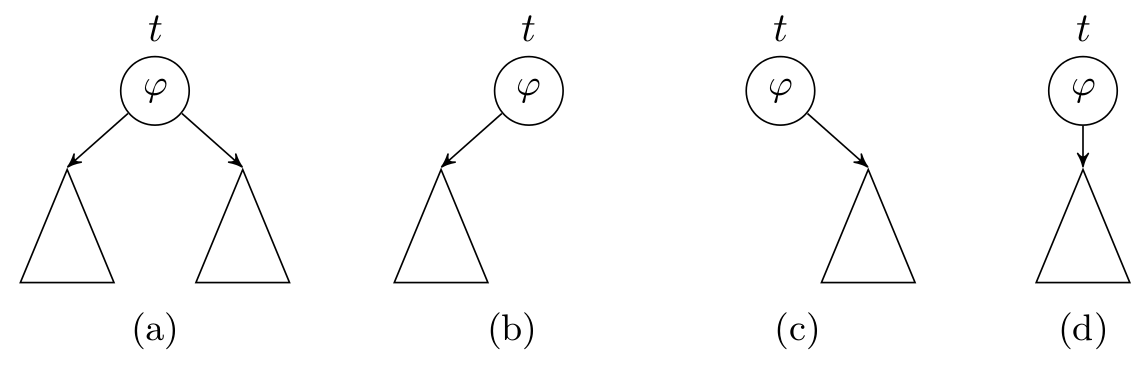
\includegraphics[width=0.9\textwidth]{figs/PTrees/ptrees.png}
	  \caption{Compact P-trees}
	\end{figure}
}

\frameT{Relative Expressivity of Preference Languages}{
	\begin{center}
		Poss-theories = ASO-rules 
		%$\subsetsim$ 
		$\subset$
			\dual{LP-trees/\dual{$\cap$/\dual{PLP-trees/\dual{$\cap$/P-trees}}}}
			$\subset$ ASO-theories
	\end{center}
}

\frameT{Computational Complexity Results}{
	{\sc DomTest}: is it that $o \succeq_T o'$ in P-tree $T$?\\
	{\sc OptTest}: is outcome $o$ optimal w.r.t $T$?\\
	{\sc OptProp}: is there an optimal outcome $o$ w.r.t $T$ st $o \models \alpha$?
	
	\begin{figure}
		\centering

	  \begin{tabular}[0.5\textwidth]{ | c | c | c | c | }
	    \hline
	     & {\sc DomTest}& {\sc OptTest} & {\sc OptProp} \\
			\hline
			LP-tree & P & P & P \\
			\hline
			\pbox{20cm}{ASO-rule/ \\ Poss-theory} & P & coNP-c & $\deltap{2}$($P^{NP}$) \\
	    \hline
	    \tbf{P-tree} & \tbf{P} & \tbf{coNP-c}\fn{The complement problem is reduced from the SAT problem.}
				& \tbf{$\deltap{2}$($P^{NP}$)-c}\fn{The problem is reduced from the Maximum Satisfying 
																					Assignment (MSA) problem.}\\
			\hline
			ASO-theory & P & coNP-c & $\sigmap{2}$($NP^{NP}$)-c \\
	    \hline
			%ACP-net & NP-hard & P & P \\
	    %\hline
			%CCP-net & PSPACE-c & PSPACE-c? & PSPACE-c? \\
	    %\hline
	  \end{tabular}

		\caption{Computational complexity results}

	\end{figure}
}

\frameT{Partial Lexicographic Preference Trees (PLP-Tree)}{
	A \tit{PLP-tree} over $\CD(\cI)$ is a tree, where
	\begin{enumerate}
		\setlength\itemsep{0em}
		\item every node $t$ is labeled with an attribute $\Attr(t)$ in $\cI$ and
					a conditional preference table $\CPT(t)$,
	  \item every non-leaf node $t$ has either one unlabeled outgoing edge or multiple
					outgoing edges labeled, each labeled by some value in $\Dom(\Attr(t))$, and
		\item every attribute appears \tit{at most} once on every branch.
	\end{enumerate}
}

\frameT{Partial Lexicographic Preference Trees (PLP-Tree)}{
	\begin{figure}[ht!]
	  \centering
	    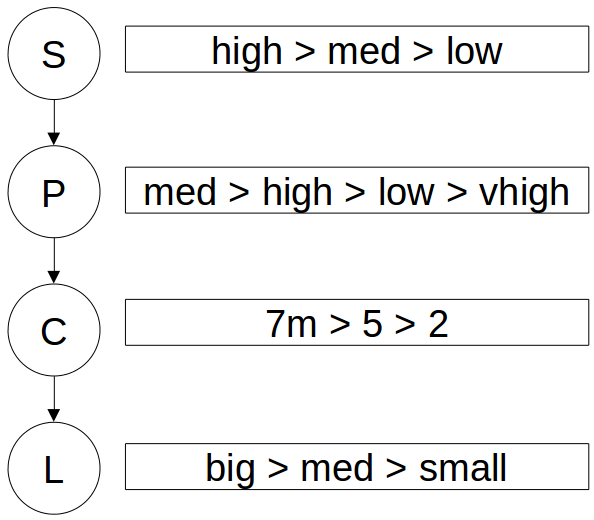
\includegraphics[width=0.4\textwidth]{figs/Cars/uiuptree.png}
	  \caption{A UIUP PLP-tree}
	\end{figure}

	According to this UIUP PLP-tree, \tit{Car1} is preferred to \tit{Car2}.
}

\frameT{Partial Lexicographic Preference Trees (PLP-Tree)}{
	\begin{figure}[ht!]
	  \centering
	    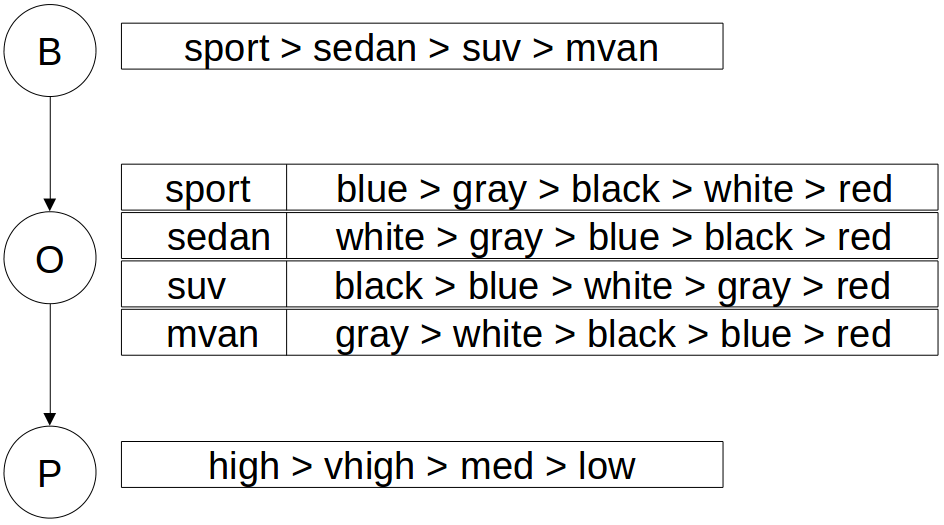
\includegraphics[width=0.65\textwidth]{figs/Cars/uicptree.png}
	  \caption{A UICP PLP-tree}
	\end{figure}

	According to this UICP PLP-tree, \tit{Car2} is preferred to \tit{Car1}.
}

\frameT{Partial Lexicographic Preference Trees (PLP-Tree)}{
	\begin{figure}[ht!]
	  \centering
	    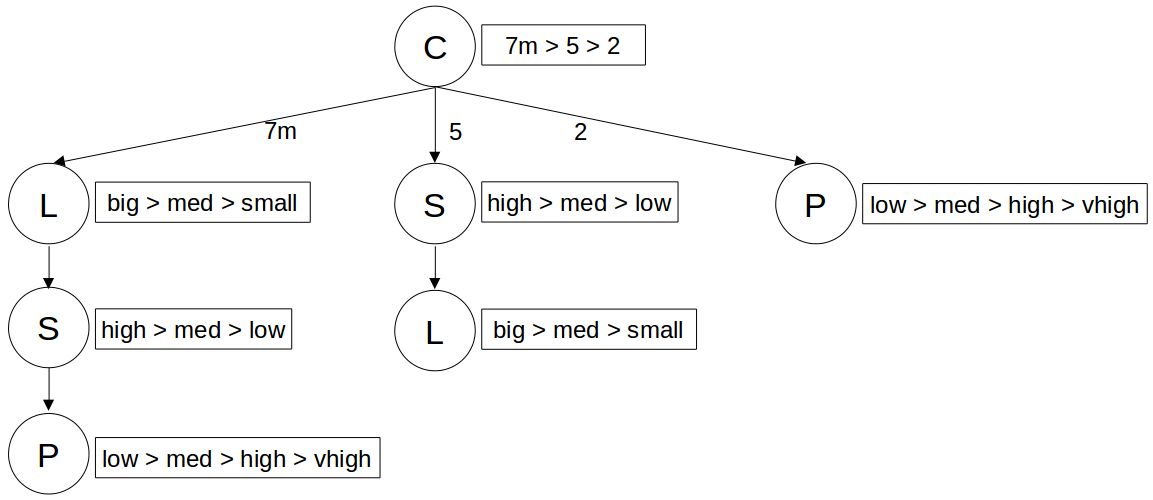
\includegraphics[width=0.9\textwidth]{figs/Cars/ciuptree.png}
	  \caption{A CIUP PLP-tree}
	\end{figure}

	According to this CICP PLP-tree, \tit{Car1} is preferred to \tit{Car2}.
}

\frameT{Partial Lexicographic Preference Trees (PLP-Tree)}{
	\begin{figure}[ht!]
	  \centering
	    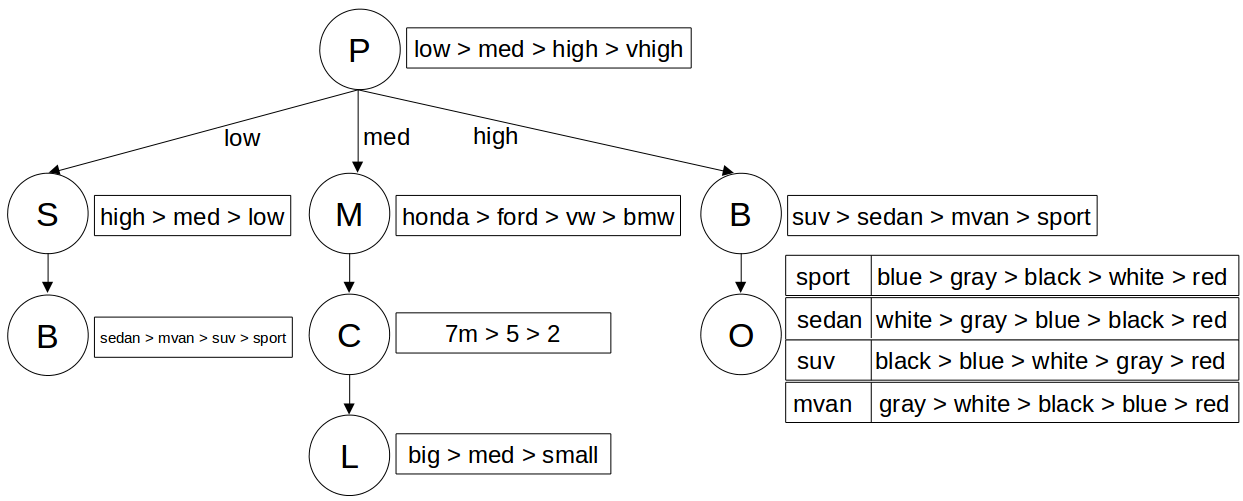
\includegraphics[width=0.9\textwidth]{figs/Cars/cicptree.png}
	  \caption{A CICP PLP-tree}
	\end{figure}

	According to this CICP PLP-tree, \tit{Car1} is preferred to \tit{Car2}.
}

\frameT{Lexicographic Preference Trees (LP-Trees)}
{
  \begin{enumerate}
    \item An \tit{LP-tree} $\cL$ over $\CD(\cI)$ is a PLP-tree, where
    \begin{itemize}
      \item each attribute appears \tbf{exactly once} on every path from the root to a leaf.
    \end{itemize}
  \end{enumerate}
}
